\documentclass[reprint,english,notitlepage]{revtex4-2}
\usepackage{amsmath}
\usepackage[mathletters]{ucs}
\usepackage[utf8x]{inputenc}
\usepackage[english]{babel}
\usepackage{esint}
\usepackage{physics,amssymb}
\usepackage{graphicx}
\usepackage{xcolor}
\usepackage{hyperref}
\usepackage{listings}
\usepackage{subfigure}
% \usepackage[style=science, backend=biber]{biblatex}
% \addbibresource{References_Part_4.bib} TODO: Slett før innlevering
\hypersetup{
    colorlinks,
    linkcolor={red!50!black},
    citecolor={blue!50!black},
    urlcolor={blue!80!black}}

\lstset{inputpath=,
    backgroundcolor=\color{white!88!black},
    basicstyle={\ttfamily\scriptsize},
    commentstyle=\color{magenta},
    language=Python,
    morekeywords={True,False},
    tabsize=4,
    stringstyle=\color{green!55!black},
    frame=single,
    keywordstyle=\color{blue},
    showstringspaces=false,
    columns=fullflexible,
    keepspaces=true}

\begin{document}

\title{Preparing For The Landing}
\author{Oskar Idland \& Jannik Eschler}
\date{\today}
\affiliation{Institute of Theoretical Astrophysics, University of Oslo}

\begin{abstract}
    This is an abstract \colorbox{red}{Complete this summary at the end of the paper}
\end{abstract}
\maketitle
\section{Introduction} \label{sec:introduction}
\colorbox{red}{To be added if evaluation includes this part}
\section{Theory} \label{sec: theory}
\colorbox{red}{To be added if evaluation includes this part}
\section{Method} \label{sec: method}
\colorbox{red}{To be added if evaluation includes this part}
\section{Results} \label{sec: results}
\onecolumngrid
\subsection{Spectral Analysis of the Atmosphere} \label{ssec: Analysis results}
\begin{table}[h!] \label{tab: Spec anal}
  \begin{tabular}{|c|*{4}{c|}}    
    \hline
    Gas  &Wavelength (nm) &Min. Flux &Temperature (K) &Doppler Shift (nm) \\
    \hline
    $ O_{2} $ &632 &0.90 &150.0 &8.96e-03 \\
    \hline
    $ O_{2} $ &690 &0.87 &450.0 &1.24e-02 \\
    \hline
    $ O_{2} $ &760 &0.93 &450.0 &1.58e-02 \\
    \hline
    $ H_{2}O $ &720 &0.95 &150.0 &2.27e-02 \\
    \hline
    $ H_{2}O $ &820 &0.91 &189.2 &1.48e-02 \\
    \hline
    $ H_{2} O$ &940 &0.87 &424.4 &7.55e-03 \\
    \hline
    $ CO_{2} $ &1400 &0.90 &450.0 &2.70e-02 \\
    \hline
    $ CO_{2} $ &1600 &0.93 &250.0 &5.56e-02 \\
    \hline
    $ CH_{4} $ &1660 &0.90 &150.0 &6.57e-03 \\
    \hline
    $ CH_{4} $ &2200 &0.90 &450.0 &4.36e-02 \\
    \hline
    $ CO $ &2340 &0.97 &216.7 &2.74e-02 \\
    \hline
    $ N_{2}O $ &2870 &0.97 &183.3 &3.32e-02 \\
    \hline
    \end{tabular}
  \end{table}
  \newpage
  \clearpage
  \begin{figure}[h!]  
    \centering
    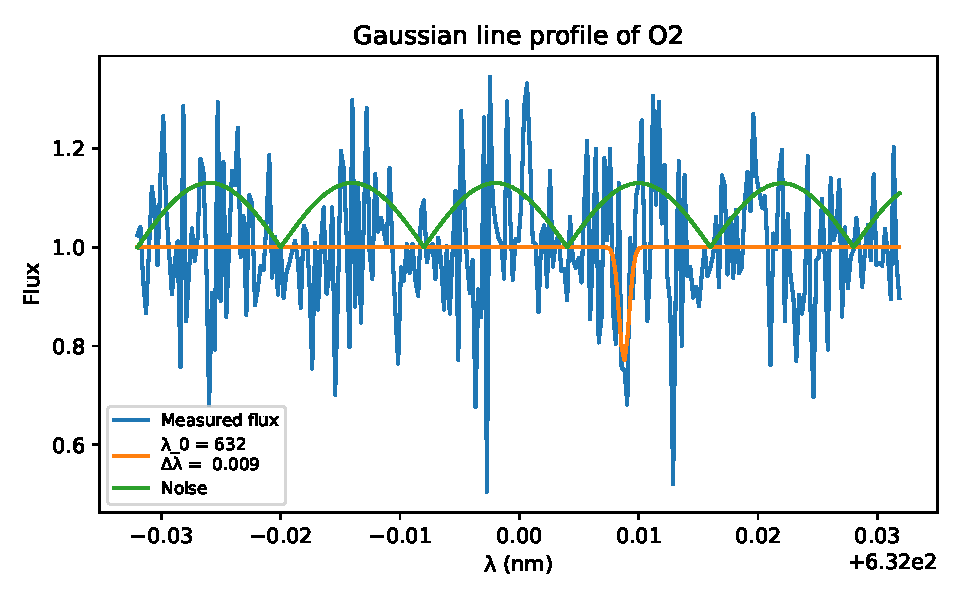
\includegraphics[scale =.3]{Figures/O2 632.pdf}
    \caption{Flux Data and Spectral Line Analysis}
    \label{fig: O2 632}
\end{figure}

\begin{figure}[h!]  
    \centering
    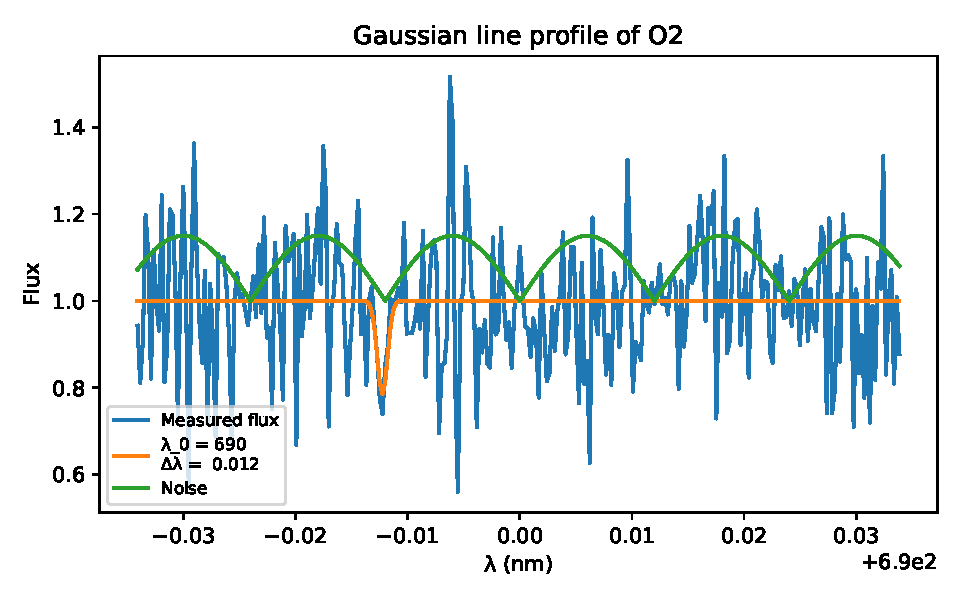
\includegraphics[scale =.3]{Figures/O2 690.pdf}
    \caption{Flux Data and Spectral Line Analysis}
    \label{fig: O2 690}
\end{figure}

\begin{figure}[h!]
  \centering
  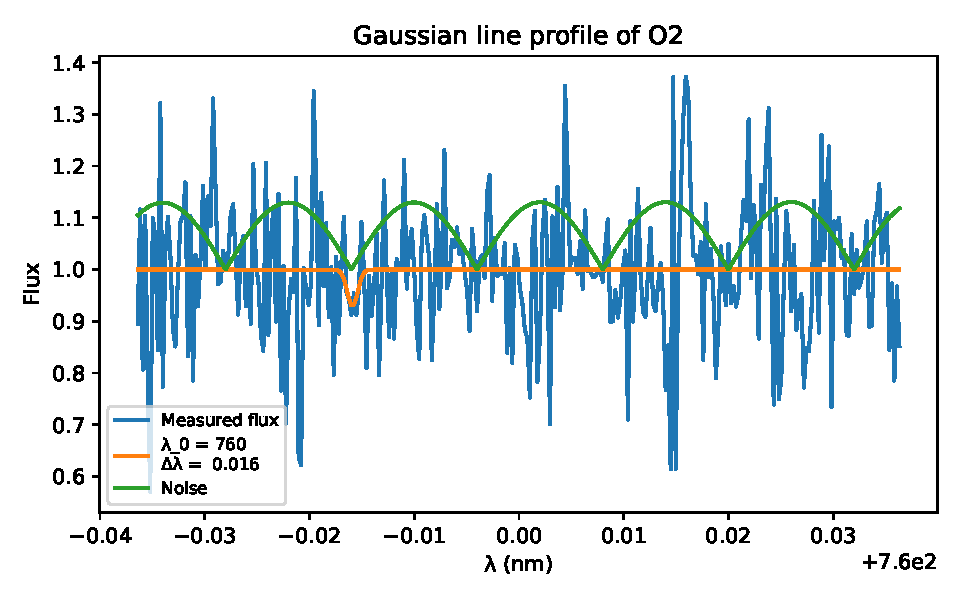
\includegraphics[scale =.3]{Figures/O2 760.pdf}
  \caption{Flux Data and Spectral Line Analysis}
  \label{fig: O2 760}
\end{figure}

\begin{figure}[h!]
  \centering
  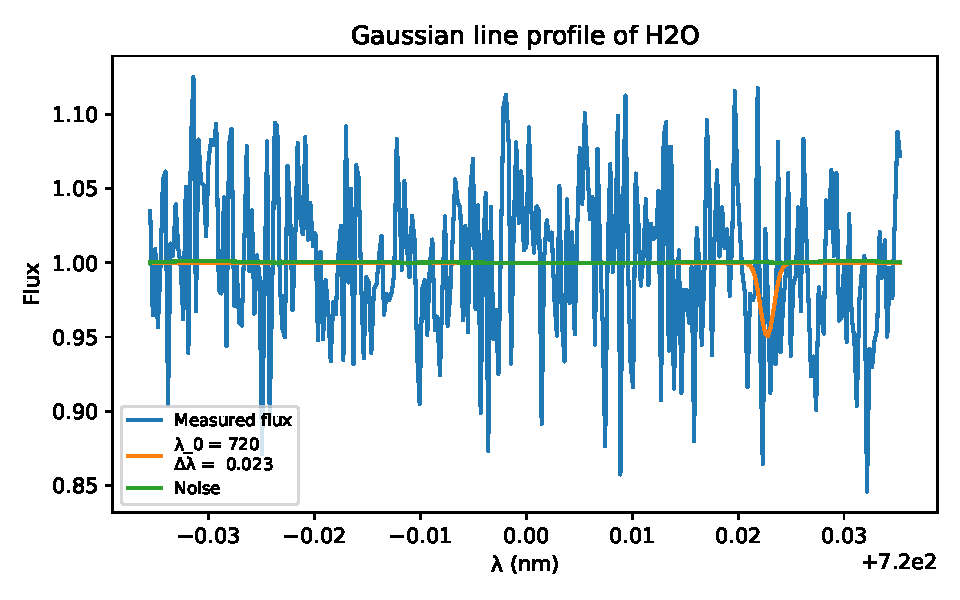
\includegraphics[scale =.3]{Figures/H2O 720.pdf}
  \caption{Flux Data and Spectral Line Analysis}
  \label{fig: H2 720}
\end{figure}

\begin{figure}[h!]
  \centering
  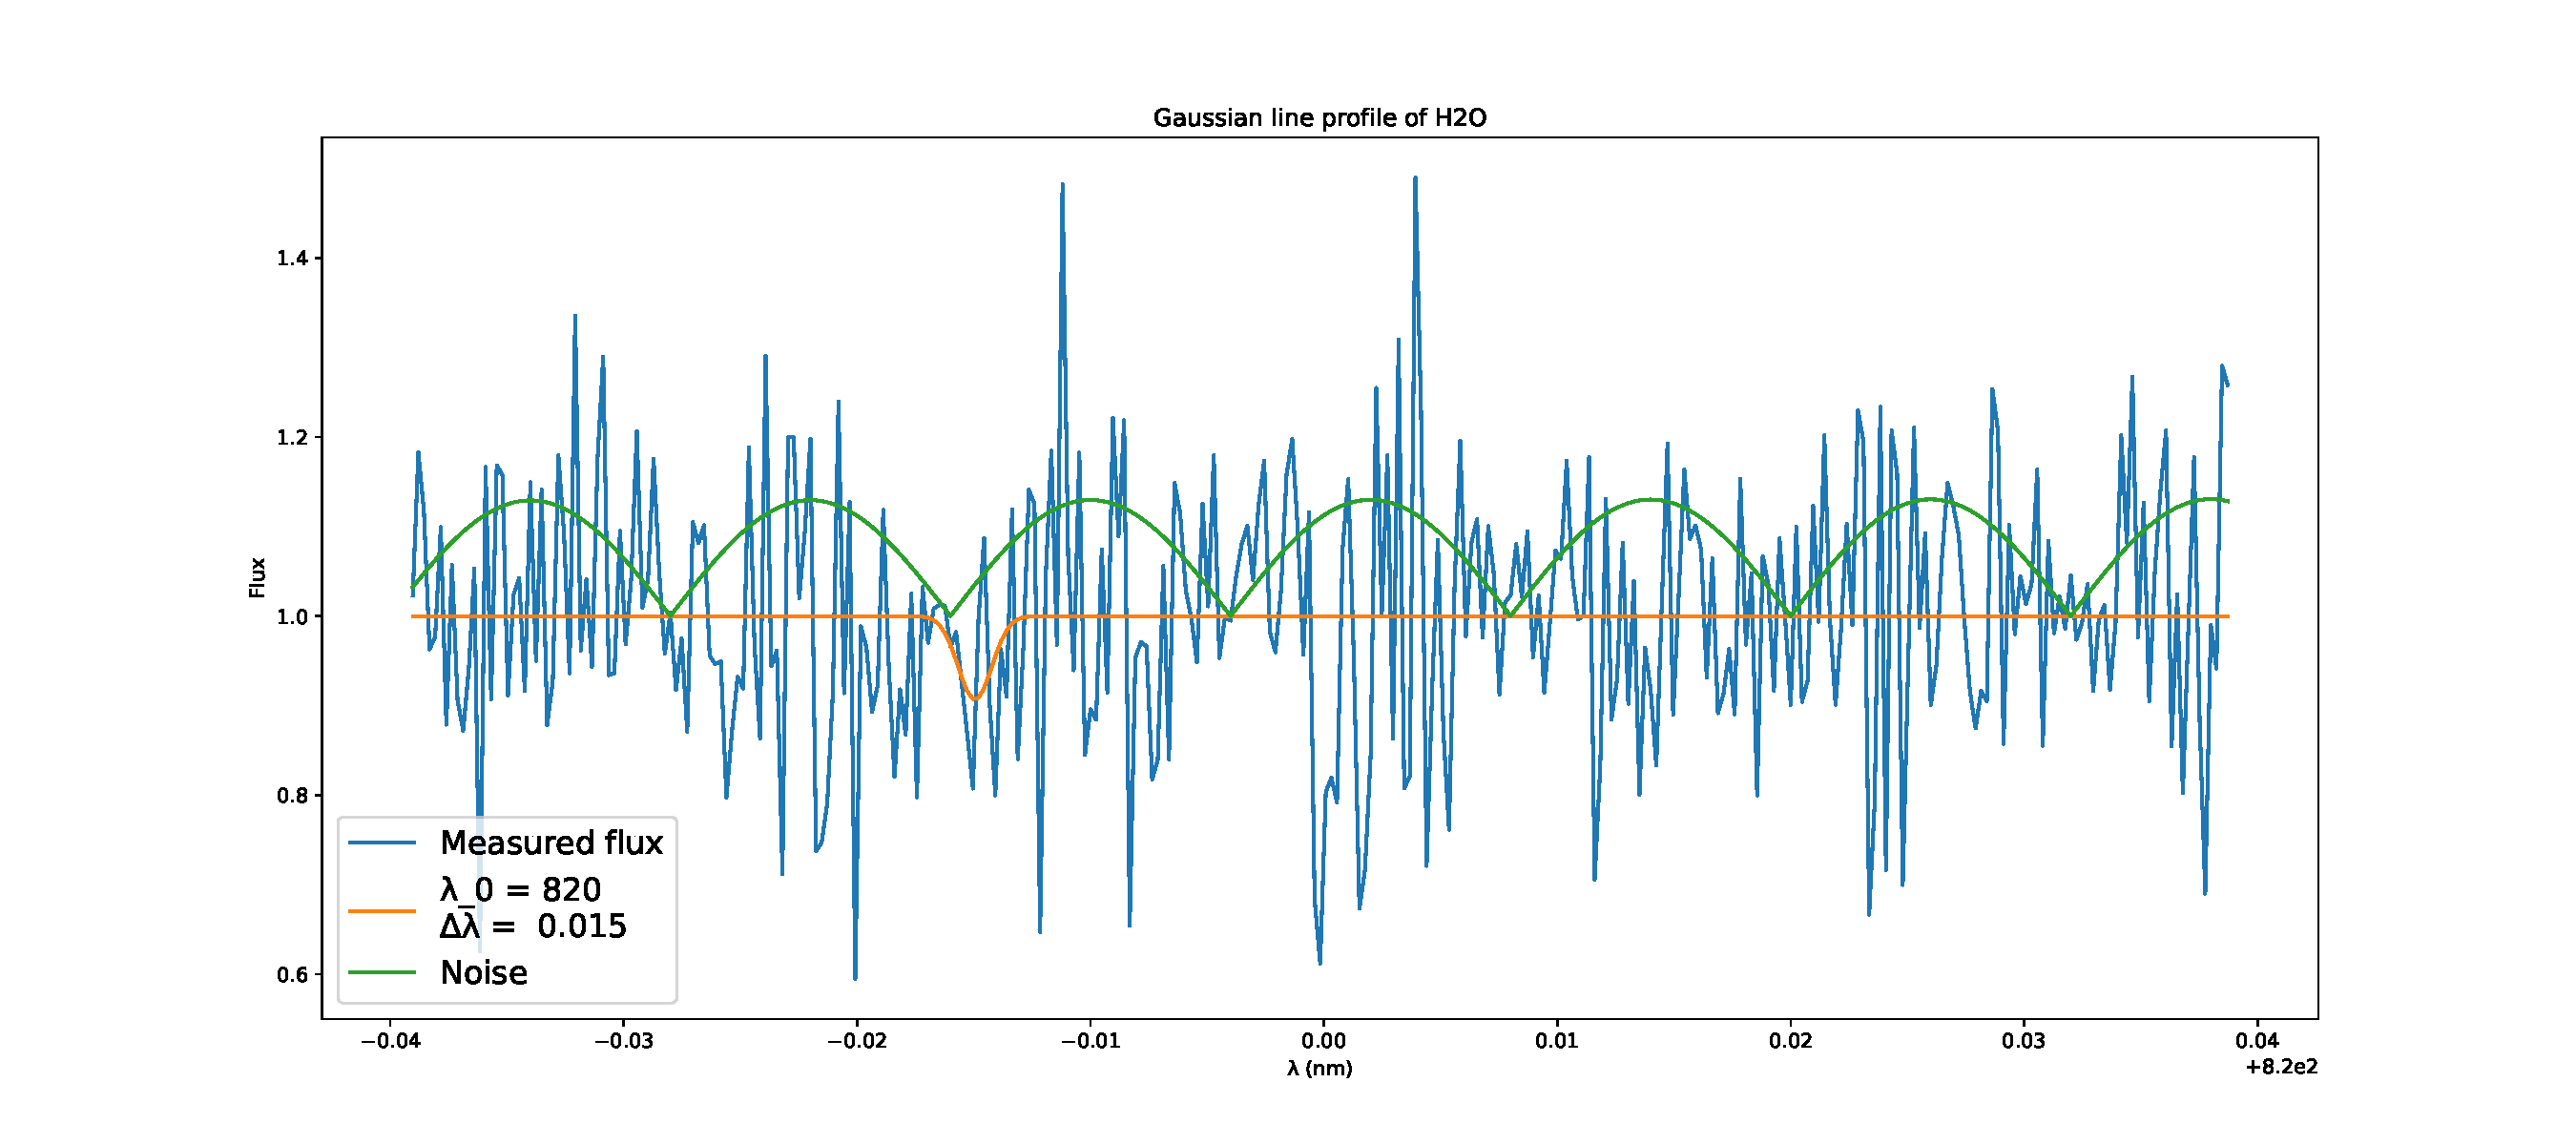
\includegraphics[scale =.3]{Figures/H2O 820.pdf}
  \caption{Flux Data and Spectral Line Analysis}
  \label{fig: H2 820}
\end{figure}

\begin{figure}[h!]
  \centering
  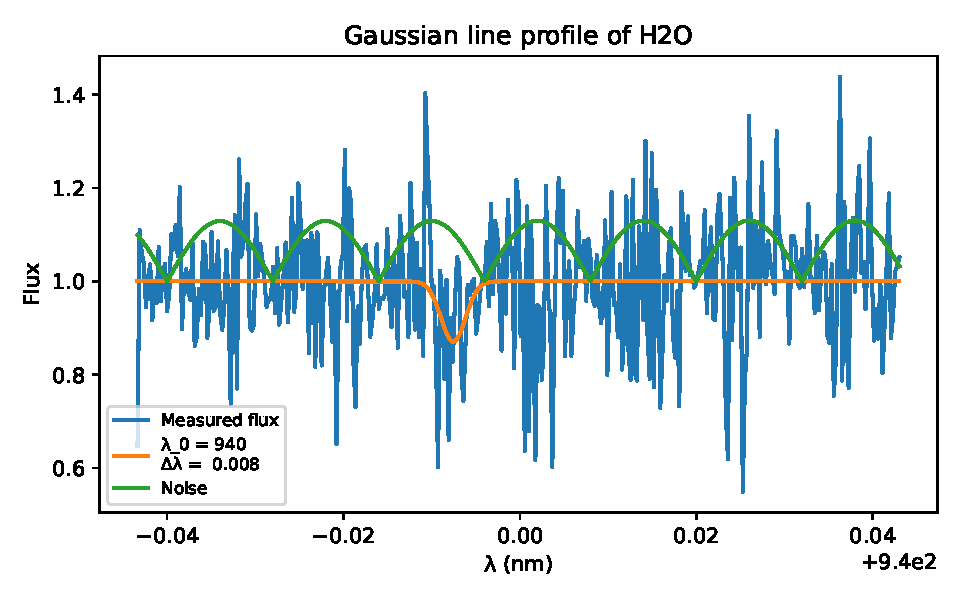
\includegraphics[scale =.3]{Figures/H2O 940.pdf}
  \caption{Flux Data and Spectral Line Analysis}
  \label{fig: H2 940}
\end{figure}

\begin{figure}[h!]
  \centering
  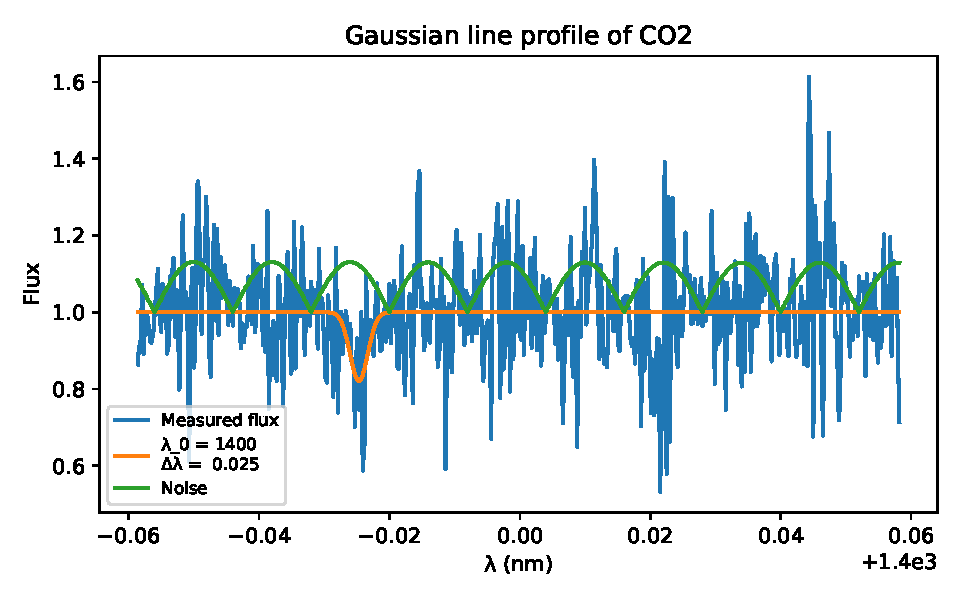
\includegraphics[scale =.3]{Figures/CO2 1400.pdf}
  \caption{Flux Data and Spectral Line Analysis}
  \label{fig: CO2 1400}
\end{figure}

\begin{figure}[h!]
  \centering
  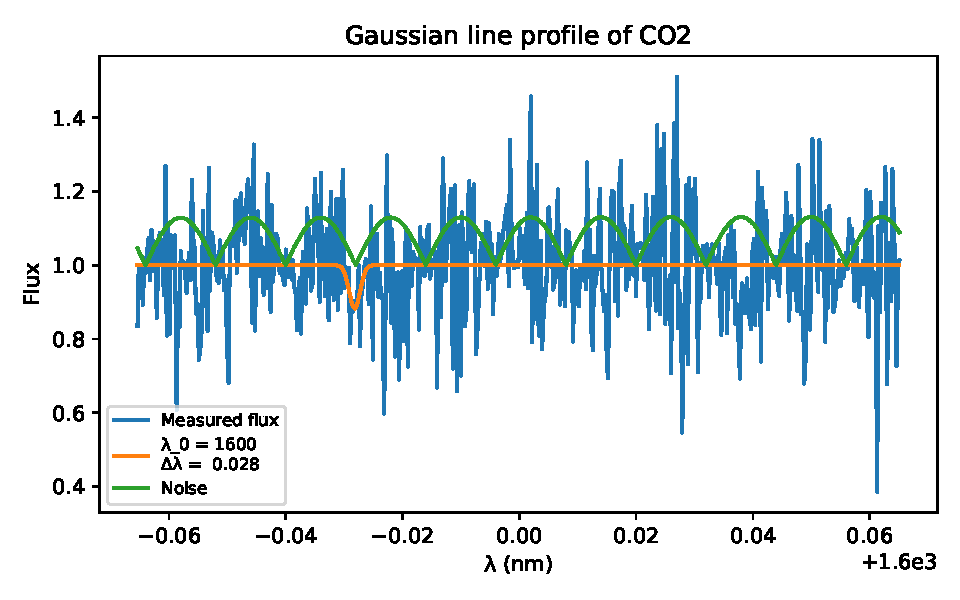
\includegraphics[scale =.3]{Figures/CO2 1600.pdf}
  \caption{Flux Data and Spectral Line Analysis}
  \label{fig: CO2 1600}
\end{figure}

\begin{figure}[h!]
  \centering
  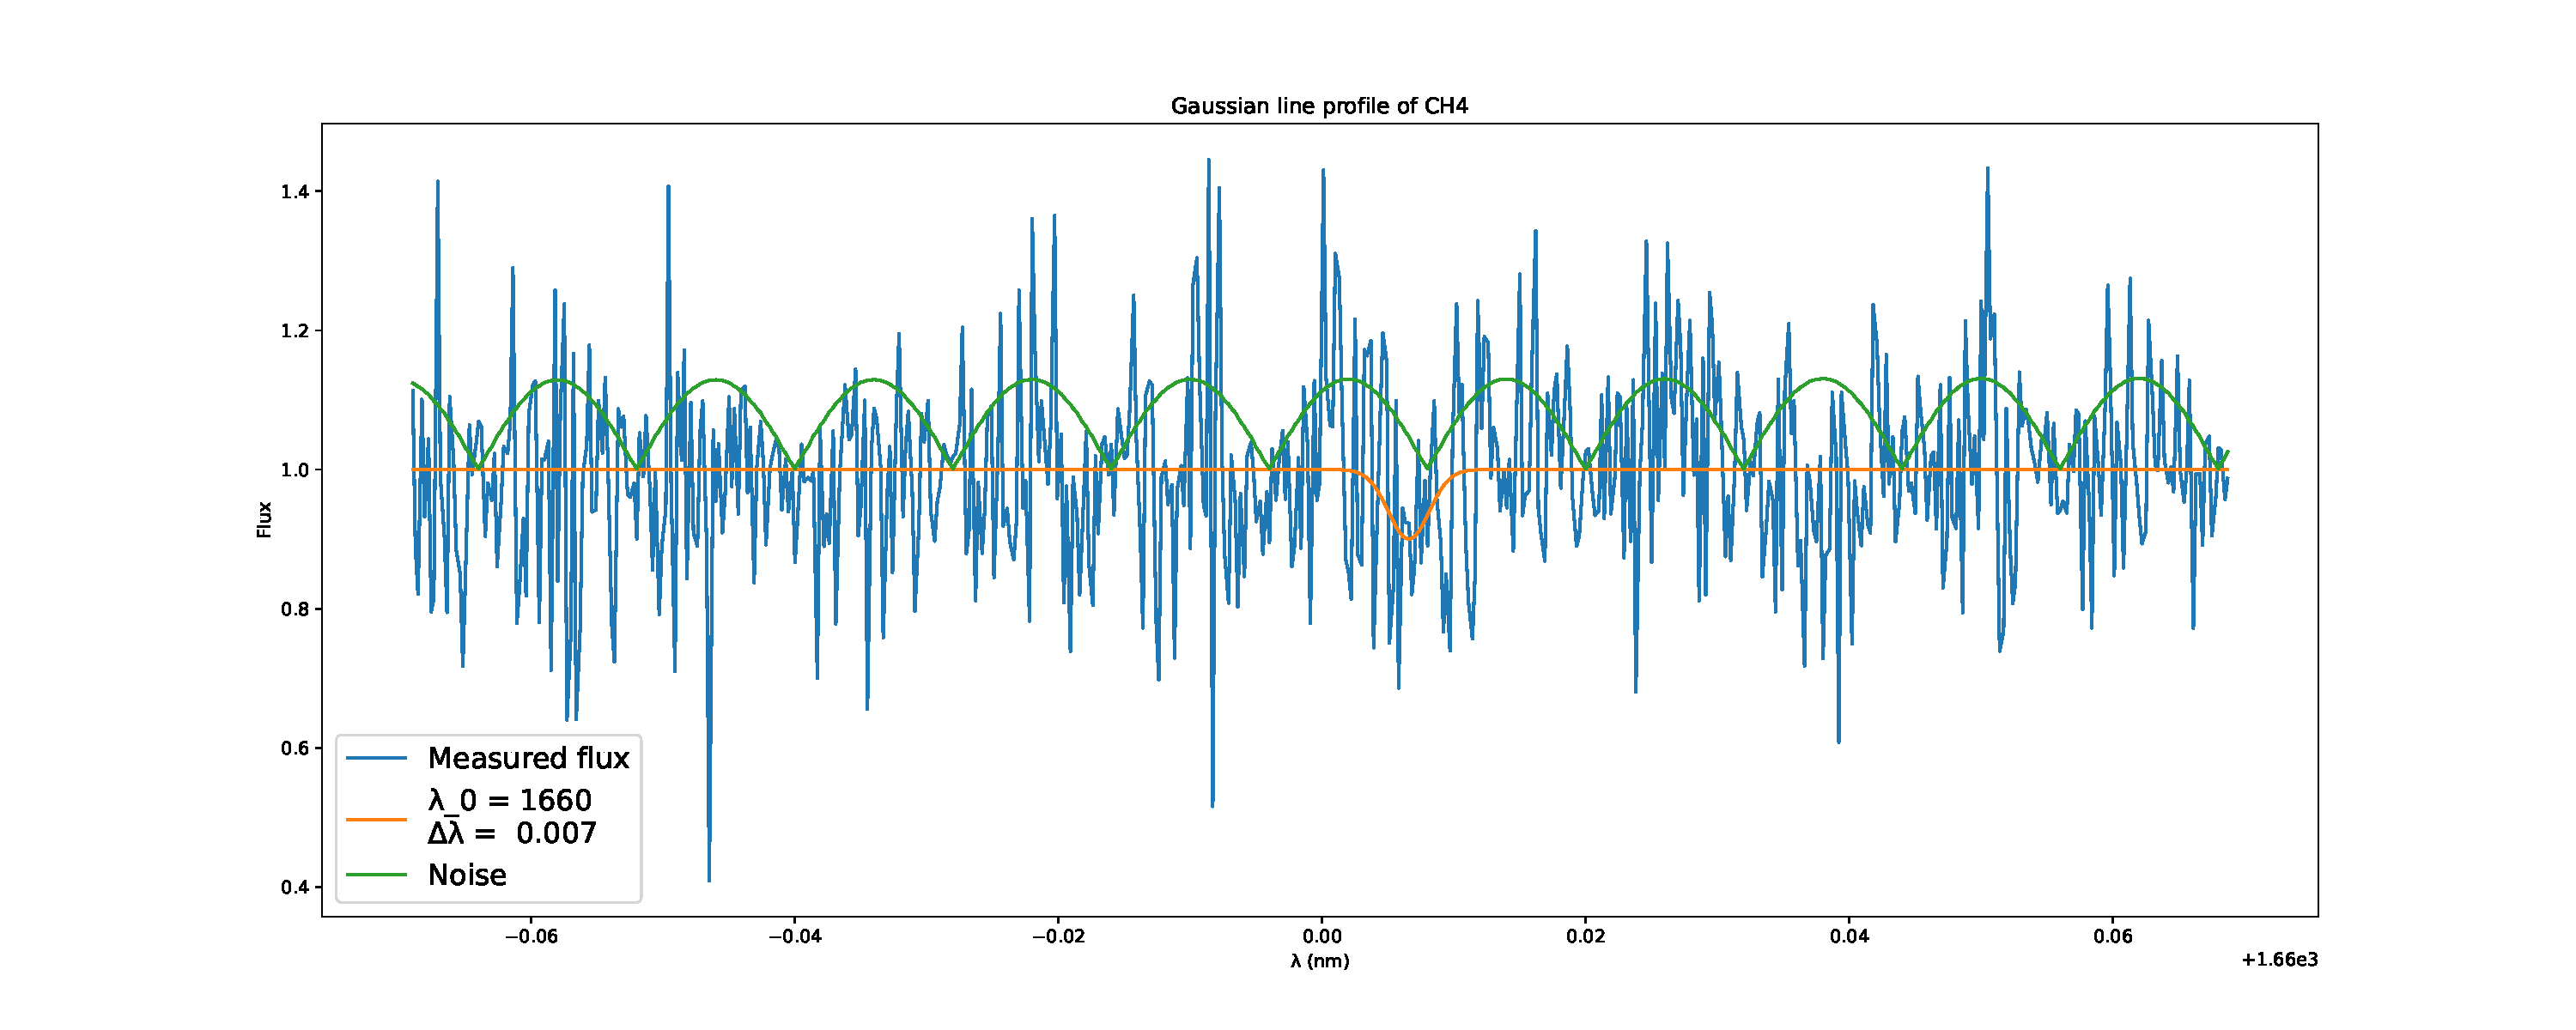
\includegraphics[scale =.3]{Figures/CH4 1660.pdf}
  \caption{Flux Data and Spectral Line Analysis}
  \label{fig: CH4 1660}
\end{figure}

\begin{figure}[h!]
  \centering
  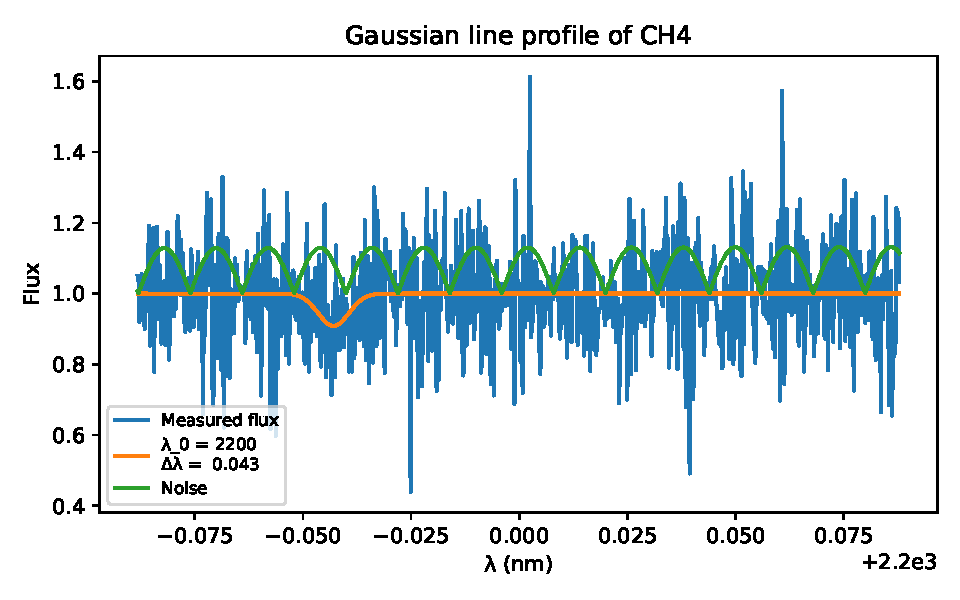
\includegraphics[scale =.3]{Figures/CH4 2200.pdf}
  \caption{Flux Data and Spectral Line Analysis}
  \label{fig: CH4 2200}
\end{figure}

\begin{figure}[h!]
  \centering
  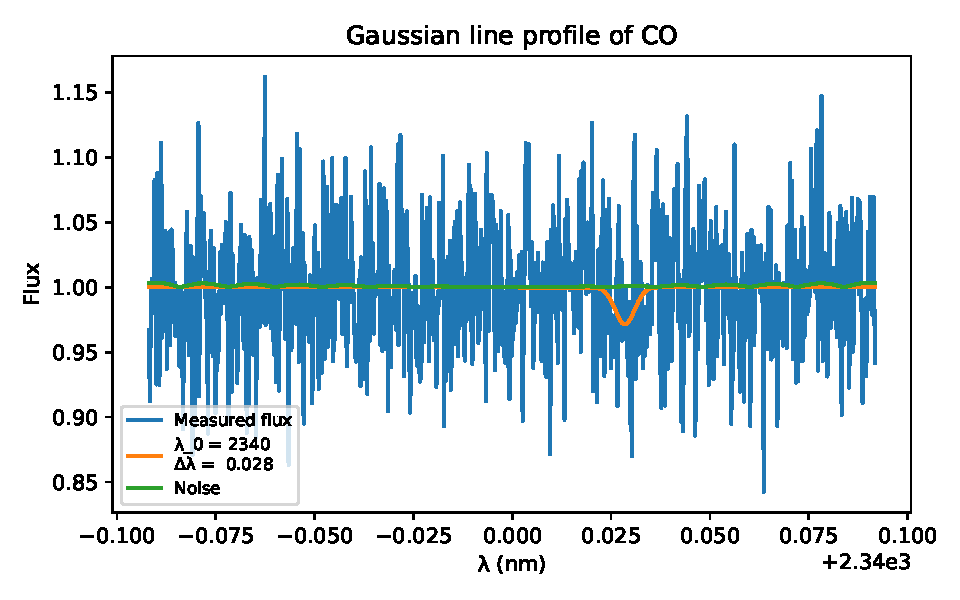
\includegraphics[scale =.3]{Figures/CO 2340.pdf}
  \caption{Flux Data and Spectral Line Analysis}
  \label{fig: CO 2340}
\end{figure}

\begin{figure}[h!]
  \centering
  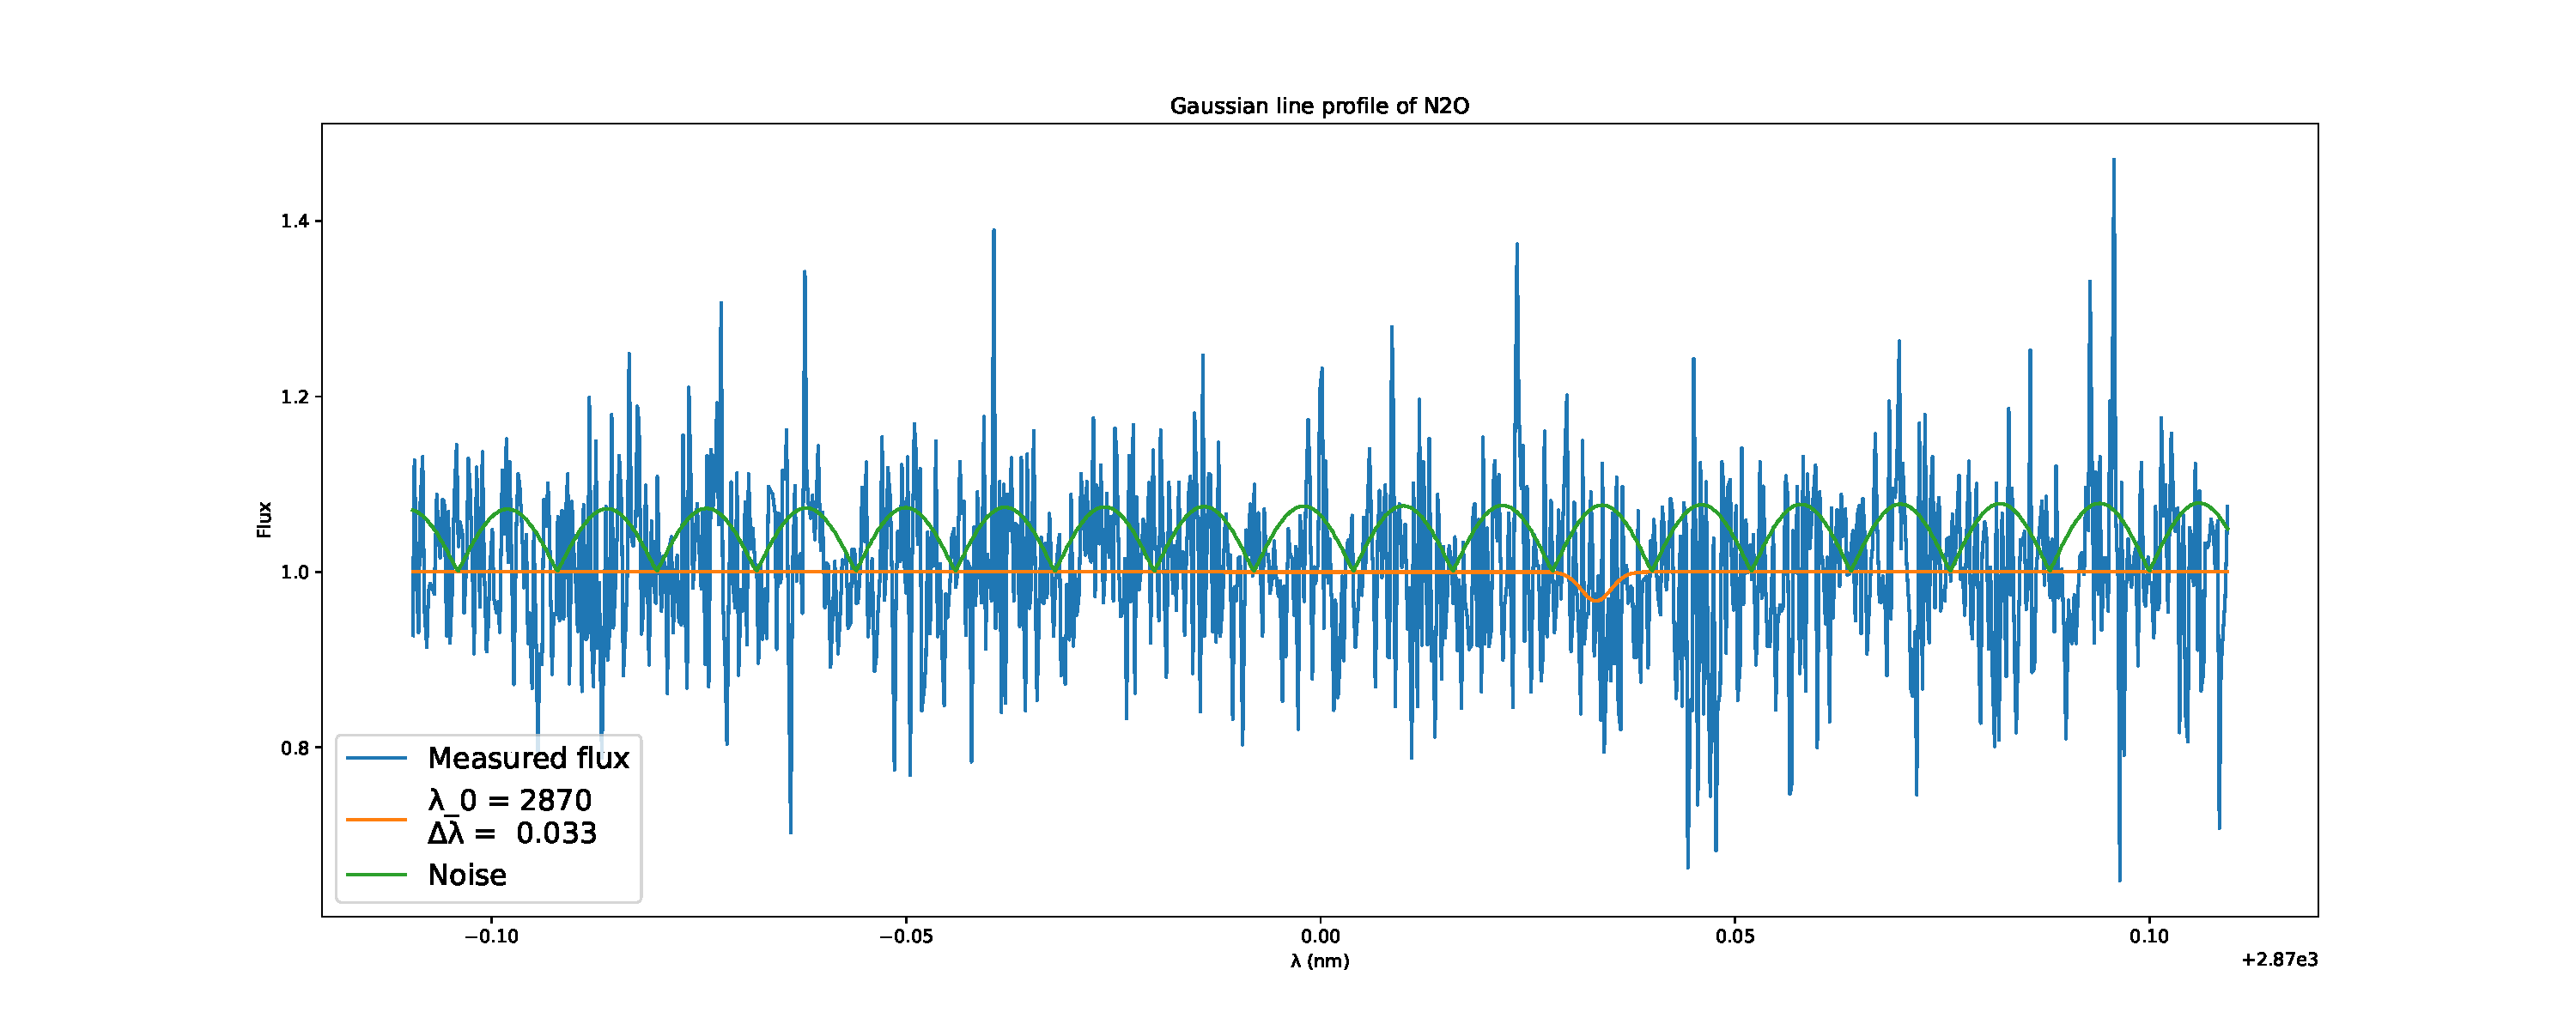
\includegraphics[scale =.3]{Figures/N2O 2870.pdf}
  \caption{Flux Data and Spectral Line Analysis}
  \label{fig: N20 2870}
\end{figure}
\clearpage
\twocolumngrid

Depicted in Figure \ref{fig: O2 632}, \ref{fig: O2 690}, \ref{fig: O2 760}, \ref{fig: H2 720}, \ref{fig: H2 820}, \ref{fig: H2 940}, \ref{fig: CO2 1400}, \ref{fig: CO2 1600}, \ref{fig: CH4 1660}, \ref{fig: CH4 2200}, \ref{fig: CO 2340} \& \ref{fig: N20 2870} are the Gaussian line profile of possible gases contained in the target planets atmosphere. Table \ref{tab: Spec anal} depicts much of the same information in addition to the temperature. 

On top of the plots we have added the noise from our data. The noise have values in the range of 0.05 to 0.15, but  For the sake of visualization we have added 0.95 as to lay the noise on top of the other data to make it easier to see its effect. 

\subsection{Model of Planet Atmosphere}
\begin{figure}[h!]
  \centering
  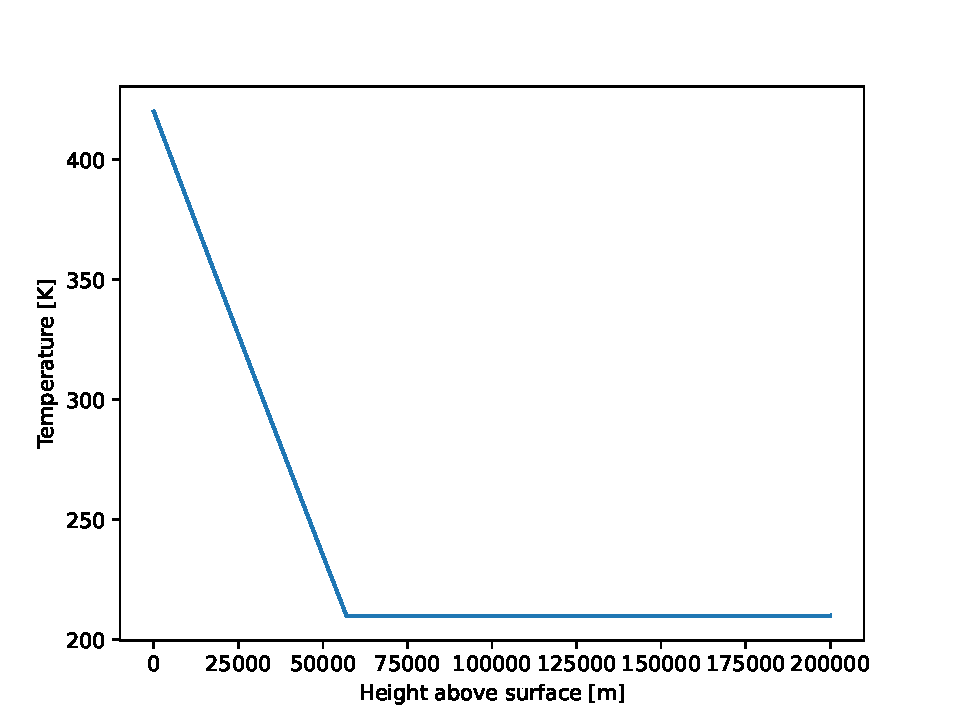
\includegraphics[scale = .4]{Figures/Temperature plot.pdf}
  \caption{Our model of the temperature as a function of meters above the surface }
  \label{fig: Temperature}
\end{figure}

\begin{figure}[h!]
  \centering
  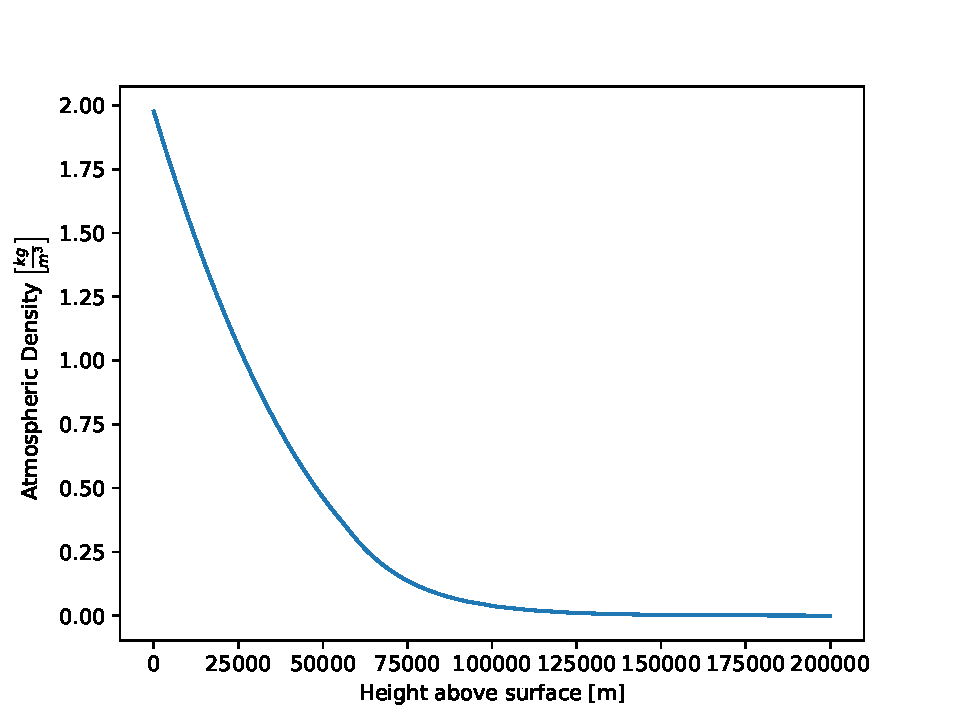
\includegraphics[scale = .4]{Figures/Density plot.pdf}
  \caption{Our model of the atmospheric density as a function of meters above the surface }
  \label{fig: Density}
\end{figure}


\section{Discussion} \label{sec: discussion}
\subsection{Spectral Line Analysis} \label{ssec: Spec Anal}
  
To filter out spectral lines which were flukes we used a multitude of criteria.

\begin{itemize}
  \item Temperature of different spectral lines in one gas
  \item Variation in the analysis with different levels of accuracy
  \item Doppler shift
  \item Amount of flux
  \item How good a fit the calculated line is in comparison to measurements
\end{itemize}

Of a real spectral line we expect the lines to have about the same temperature. This was not the case for either $ O_{2} $, $ H_2O  $, $ CO_2 $ and $ CH_4 $. We therefore doubt them being possible gases in the atmosphere.
\newline

When running our analysis we could choose whatever accuracy we wanted. As our accuracy got higher a lot of our results changed temperature drastically. This was to our advantage as it most likely meant the spectral line was a fluke. Using this as a criteria we can could be even more secure in our choice to doubt $ O_2 $, $ H_2O $ and $ CH_4 $. The temperature of $ CO $ and $ N_2O $  converged towards 217 K and 183 K respectivly as seen in table \ref{tab: Spec anal}.
\newline

The Doppler shift is quite inconsistent in most cases. We clearly observe this in $ CO_2 $, $ H_2O $ and $ CH_4 $ in which we observe the absolute shift being around 2 times as much for $ CO_2 $, 2-3 times as much for $ H_2O $ and 7 times as much for $ CH_4 $. In all other cases their are either just one line per gas or consistent results. $ O_2 $ had very consistent results. 
\newline

The flux was on the higher end of what we expected (0.7 $ →  $ 1). Only a single line of $ O_2 $ and $ H_2O $ broke through 0.90. We expect to see a lower flux for real spectral lines. The most likely candidates so far being $ N_2O $ and $ CO  $ both had a very high flux of 0.97 which makes it more uncertain they are real. 
\newline

When looking into which spectral lines fit the measured data the most we also need to take the noise into account. The more noise, the higher the likelihood of fluctuations looking like spectral lines. We will focus on the parts of the graphs where the noise is relatively low and seemingly bounces of the Gaussian line distribution. 
\subsubsection*{$ O_2 $}
The first spectral line of $O_2$ at 632 nm \ref{fig: O2 632} is not too far off the peak of the noise and has a big fluctuations all around. This seems to most likely be a fluke. 

The second spectral line of $O_2$ at 690 nm \ref{fig: O2 690} is very close to a local minima point. Comparing this to every other local minima of the noise we see our line profile gives a good match with the lowest fluctuations of all the local minimums. This seems to be a real line 

The third spectral line of $O_2$ at 760 nm \ref{fig: O2 760} is also very close to a local minima and our line profile seems like a good fit here as well. Out of all the local minima points this also seems like the most likely to contain a true line. 

Just looking at the graphs we observe oxygen giving us two seemingly good fits.  

\subsubsection*{$ H_2O $}
All the line profiles of $ H_2O $ seen in \ref{fig: H2 720}, \ref{fig: H2 820} and \ref{fig: H2 940} Are surrounded by a lot of data not matching our line profile, and do not seem like good fits. 

\subsubsection*{$ CO_2 $}
The first spectral line of $ CO_2 $ seen in \ref{fig: CO2 1400} is close to a local maxima of noise so we can not say with certainty wether or not this is a true line or just a fluke. 

The second spectral line of $ CO_2 $ seen in \ref{fig: CO2 1600} is located very close to a local minima of noise which gives us confidence in its validity, but our curve is not the best fit for the measured data. 

When taking both graphs into account it seems likely that none of the spectral lines of $ CO_2 $ are real. 

\subsubsection*{$ CH_4 $}
The first spectral line of $ CH_4 $ seen in \ref{fig: CH4 1660} is not too far off a local minima of noise, but there are a lot of measured flux above our line profile, which may point to it not being a real line after all. Our graph does not fit the measured data very well either. 

The second spectral line of $ CH_4 $ seen in \ref{fig: CH4 2200} is located in between a local minima and maxima and follows the measured data quite nicely. Its the only local minima with a dip in flux over a wide range. This might be a sign the line is real. 

Judging by its graphs its very hard to say weather or not the graphs actually represent real lines. 

\subsubsection*{$ CO $}
The spectral line of $ CO $ seen in \ref{fig: CO 2340} is surrounded by a bit different data. In this case, the noise was relatively small in comparison with the measured data. This means the noise will have less an effect on the flux. When the flux varies this much with such small amounts of noise its not very likely this is a real line. Our line profile does not match too well with the measured data either. 

\subsubsection*{$ N_2O $}
The spectral line of $ N_2O $ seen in \ref{fig: N20 2870} is located right under a local maxima which makes it more likely the measured dip in flux is a result of chance and noisy data. Looking at the rest of the graph there seems to be no dip of significance around any of the local minima. 


\section{Conclusion} \label{sec: conclusion}
\subsection{Atmosphere composition} \label{ssec: Atmpos Comp}
Judging by temperature, Doppler shift and variation in analysis it seems $ CO $ and $ N_2O $ is the only viable options. These two have the most consistent and almost equal temperature. 

Judging by the flux, $ CO $ and $ N_2O  $ are the worst option. On the other hand, $ O_2 $ and $ CH_4 $ rises as the best options. 

Judging by how good a fit our model is, we observe $ O_2 $ being the best fit by far. 

To conclude the discussion of results as seen in \ref{ssec: Spec Anal}, there is no clear candidate which checks all the boxes. We choose to consider how well a fit our model is in addition to the flux the most important factors as that is based in actual data and not our just our own calculations. The line profile seen in \ref{fig: O2 690} and \ref{fig: O2 760} matches a lot closer than the one seen in \ref{fig: O2 632}. As the temperature of the first two are equal (450 $ K $) which also matches earlier estimates made in \colorbox{red}{Jannik: Refferer til temp estimat i del 3} of the planets temperature, we will assume they are real lines. The atmosphere is therefore 100 \% $ O_2 $ with a mean molecular weight $ μ $ of 
\[
μ =   \frac{2 ⋅ 15.9994 ⋅  1.66 ⋅ 10^{-27}}{1.00794 ⋅ 1.66  ⋅  10^{-27}} = 31.75.
\]



\section{Appendix} \label{sec: appendix}

\section*{ACKNOWLEDGMENTS}   

\section*{References} \label{sec: references}

\end{document}

